\section{Background}\label{background}

This section discusses the problems with the process of developing UIs today. It also provides the theoretical backgroung by highlighting the main building blocks of the UI framework.

\subsection{Accidental and Essential Complexity}

According to Brooks there is two types of complexity: Accidental Complexity and Essential Complexity. \citep{nosilverbullet}
In software engineering, \textbf{Essential Complexity} is complexity that comes from the domain problem that we want to solve. It is inherent to the problem that the customer cares about and its solution delivers business value. \textbf{Accidental Complexity} is complexity that is caused by everything else. Compilers, distributed systems and databases are all examples of Accidental Complexity. In fact even programming languages and computers are often Accidental Complexity since they are not essential to the customer's problem.

This implies that Accidental Complexity could be eradicated in an ideal world. An example of such scenario is the executable specification: It comprises only business rules which are essential to the problem of the business, it doesn't contain any Accidental Complexity.

Ben Moseley and Peter Marks explore a general infrastructure to run specifications in their paper Out of the Tar Pit \citep{outoftarpit}.

Software engineering is itself an everlasting fight against accidental complexity. This is fact the main goal of the UI framework.

\subsection{Evolution of UI web development}\label{history}

In the early days of the Internet, websites were mostly \textbf{static files} accesses under URLs. Those files were often created manually or generated by using WYSIWYG editors. The served files were mostly styles (CSS), static assets and markup that the browsers had to render.

\textbf{Dynamically generated} content became popular with the rise of PHP. Websites were now able to show different things to each user based on previous interaction. The files that were served to the browsers were still the same static files. The markup was not hard coded anymore but dynamically rendered on the server upon user request.
\\ Developers had to work with templating languages to implement UIs that received that usually from the same server.

Websites became \textbf{truly interactive} with the introduction of AJAX. AJAX allowed the browser to asynchronously communicate with the server while the user was interacting with the website. Google was able to give search suggestions in real-time while the user was typing the search term. Websites were still rendered on the server but the served files additionally contained JavaScript that was run by the browser.
\\ UI development involved working with templating languages, styling and a small amount of programming.

The amount of interactive elements on websites and their \textbf{complexity increased}. What was once a text input field with real-time suggestions became a full-text search interface with complex filtering and sorting options. The standardization of browser APIs was in the early stages and developers had to spend effort to create a consistent user experience across various browsers.
\\ Tools like jQuery emerged that provided a single interface for multiple browsers. The websites were still dynamically rendered on the server and were enriched in the browser by running JavaScript.

The first applications appeared providing a user experience in the browser similar to the one of fat desktop applications. The files that the server sent to the browser were mostly JavaScript. The browser ran that JavaScript application to render the website and to react on user input. It communicated with the server using AJAX and the website was not rendered on the server anymore. Instead a single website was served on which the application lifecycle took place. \textbf{Single page applications} (SPA) were born.
\par Development of UIs has drastically changed because the UI was part of an application that had its own lifecycle. Development of the server and the client application often took place separated. The HTTP API played the role of an informal contract between client and server.

\subsection{Document Object Model}\label{documentobjectmodel}

The Document Object Model (DOM) is a programming API for HTML and XML documents. It defines the logical structure of documents and the way a document is accessed and manipulated. \citep{domintro} \\ We consider following HTML document:

\lstset{language=XML}
\begin{lstlisting}[caption=HTML document of a table, label=htmloftable]
<table>
  <rows>
    <tr>
      <td>Walter</td>
      <td>White</td>
    </tr>
    <tr>
      <td>Saul</td>
      <td>Goodman</td>
    </tr>
  </rows>
</table>
\end{lstlisting}

The DOM representation of that table looks as follows:

\begin{figure}[!htb]
  \center{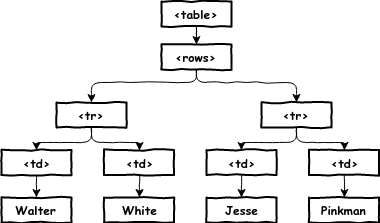
\includegraphics[width=250pt]
    {images/dom.png}}
  \caption{The DOM is a tree data structure representing an HTML document.}
\end{figure}

It is worth to note that the DOM API is imperative. The developer has to tell the DOM how to achieve a certain transformation by providing a sequence of DOM operations. An example operation would be the removal of a node. Considering operations on the document as string, the DOM provides better developer ergonomics.

This process of creating the DOM of a document we call \textbf{rendering}. This is not to be confused with the rendering taking place in a web browser. There the creation of the DOM is just one step of the whole rendering process.

\subsection{UI web development today}\label{uidevelopmenttoday}

Some UI parts are increasingly rendered on the server again, mainly for performance reasons and search engine optimization. It is common to have a \textbf{frontend} team working on the client and a \textbf{backend} team working on the server. The frontend team makes sense of the data that comes from the server either manually or in the best case using some form of HTTP API documentation.
\\ There are efforts like Swagger or OpenAPI to formalize and standardize documentation of HTTP APIs. Often documentation can be generated to a certain extent, so the overhead to keep it up-to-date is small. Documentation helps \textbf{humans} (frontend team) to understand the data.
\\ That interpretation of the meaning of the incoming data is hard coded into the client and the UI. This causes strong coupling of the client to the data and therefore to the server. The client can not be re-used in some other \textbf{context}.

\subsubsection{Lack of context}\label{datahumanmachine}

We picture a scenario in everyday life where two good friends meet. One of them says: \textit{Have you heard about Frank? He recently got married.} Chances are high the other one knows multiple people named \textbf{Frank}. Being a human, he is able to map the name \textbf{Frank} to the person the other one is referring to. He is able to do so, because that conversation has an implicit context. That context is the intersection of the sets of people \textbf{both know} who might get married.
\par Exactly the same thing happens frequently in software development, especially in data exchange. A frontend developer looks at either all HTTP routes of an API or glances over the documentation. Sometimes he is able to \textbf{infer} the domain model because of his personal experiences as a human. If that developer is not familiar with the domain at all, maybe because the domain is niche, he has trouble understanding the data coming from the server. He perceives development to be difficult and he is not able to put the data being exchanged into a \textbf{context}.
\par What makes life of a human developer hard, poses an insurmountable obstacle to a machine. A machine doesn't have dozens of years of life experience to draw from when trying to understand data.\footnote{Here we talk about machines in the sense of contemporary information systems. Systems that are able to learn are deliberately ignored as they haven't been proven to be useful in this context.} The machine has to be fed a context together with the data it should understand. In traditional web UI development that context is hard coded into the client and the UI. We believe that the majority of work done in UI development could be eliminated by \textbf{exchanging data that has meaning attached to it}.

\subsection{Web components}\label{webcomponents}

In recent years an approach to rendering UIs became popular which we will call \textbf{component based} rendering. This paragraph analyzes the reason why this approach to UI development gained popularity.

\subsubsection{React}\label{sec:react}

In 2013 Facebook released a library called React, which today is one of the main tools for web development. It was one of the first libraries to encourage the usage of \textbf{web components}. Due to its widespread adoption in web development it caused a paradigm shift.

React encourages the thinking of UIs as a composition of \textbf{web components}. The UI developer doesn't touch the DOM manually and merely provides data to React. This is a declarative approach where the developer states \textbf{what} the UI looks like not \textbf{how} the UI should be rendered. \\
Most importantly, React models the problem of UI rendering as function application. This insight leads to small re-usable components which has various benefits.

\begin{figure}[!htb]
  \center{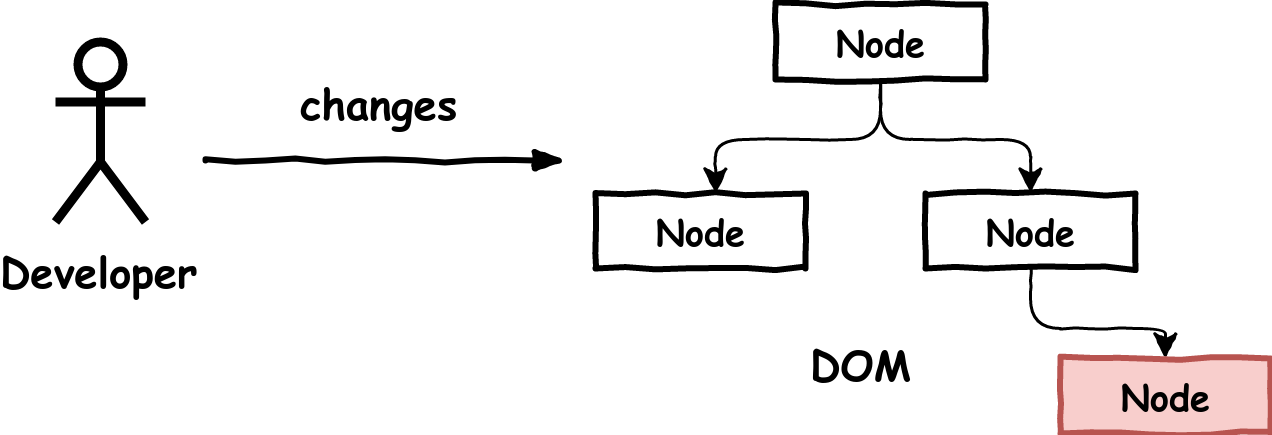
\includegraphics[width=250pt]
    {images/ui-imperative.png}}
  \caption{Imperative development: Developer works directly with DOM.}
\end{figure}

\begin{figure}[!htb]
  \center{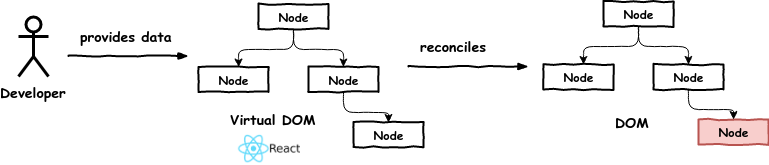
\includegraphics[width=380pt]
    {images/ui-declarative.png}}
  \caption{Declarative development: Developer provides data and React takes care of the DOM.}
\end{figure}

The markup output of a component depends only on its data input. This allows to understand the change in the output when changing the input, the component is \textbf{easy to reason about}. It can be \textbf{tested easily in isolation} because there are no other dependencies than the data input. Analogous to function composition, such web components can be \textbf{composed} to larger UIs. Because web components are designed to be self-contained, they have high cohesion which makes them usable in multiple contexts. That means a good code \textbf{reuse can be achieved}.

\subsubsection{Templates vs. Components}

The benefits of web components become apparent when we analyze UI development before web components took over. It was common to render markup dynamically on the server and send it over to the browser where some JavaScript got executed that enhances the rendered DOM. \\
On the server typically some templating language was used. Templating languages resemble simple programming languages as they provide control structures and variables together with primitives to output markup. These templates are evaluated with some input data in a template rendering step. The output of that templating step is markup. Compared to components they have major drawbacks.

Firstly, templating languages are a source of complexity. The final user of a website or the customer of a software project doesn't care about templating languages. This makes them a source of \textbf{Accidental Complexity}. They have often powerful primitives to filter collections or sort sequences or format dates. This enlarges the technology stack and the learning curve. Questions like \textit{how does the evaluation of a template happen?} or \textit{how can I debug the evaluation process} may arise at some point during development. \\
They are often used together \textbf{models} - abstractions that contain business logic. There is a risk that business logic creeps into templates which makes changes harder and more expensive.

Secondly, templates separate things that conceptually belong together. The developers of React have famously stated:
\begin{quote}
\textit{Templates separate technologies, not concerns.}
\end{quote}
We consider the UI of an issue tracking system where an issue has a status that can be changed. \\ A component representing that issue contains the \textbf{markup}, the \textbf{styling} and the \textbf{business logic} to change its status. That component is self-contained, it can be used in isolation and in various contexts. \\
A template on the other hand only takes care of creating markup. It relies on a model to provide the data and behavior and on a style sheet providing the styling.
Separation of markup, styling and business logic is done in the name of \textbf{encapsulation}. None of these could exist on their own in a sensible way because they contribute to the same thing. There is a technological and conceptual dichotomy. The main contribution of components is the acknowledgment that the conceptual one is more important since the technological one can be solved with tooling. This is the reason why components provide a higher level of encapsulation.

\subsection{Task based computing}

TODO human centered design, Don Norman

\subsection{Richardson Maturity Model}\label{richardsonmaturitymodel}

The web is an existence proof of a massively scalable distributed system that works really well and we might be able to take ideas from that to build integrated systems more easily. \citep{richardsonmaturitymodel} This section summarizes the blog post by Martin Fowler about the Richardson Maturity Model.

\begin{figure}[!htb]
  \center{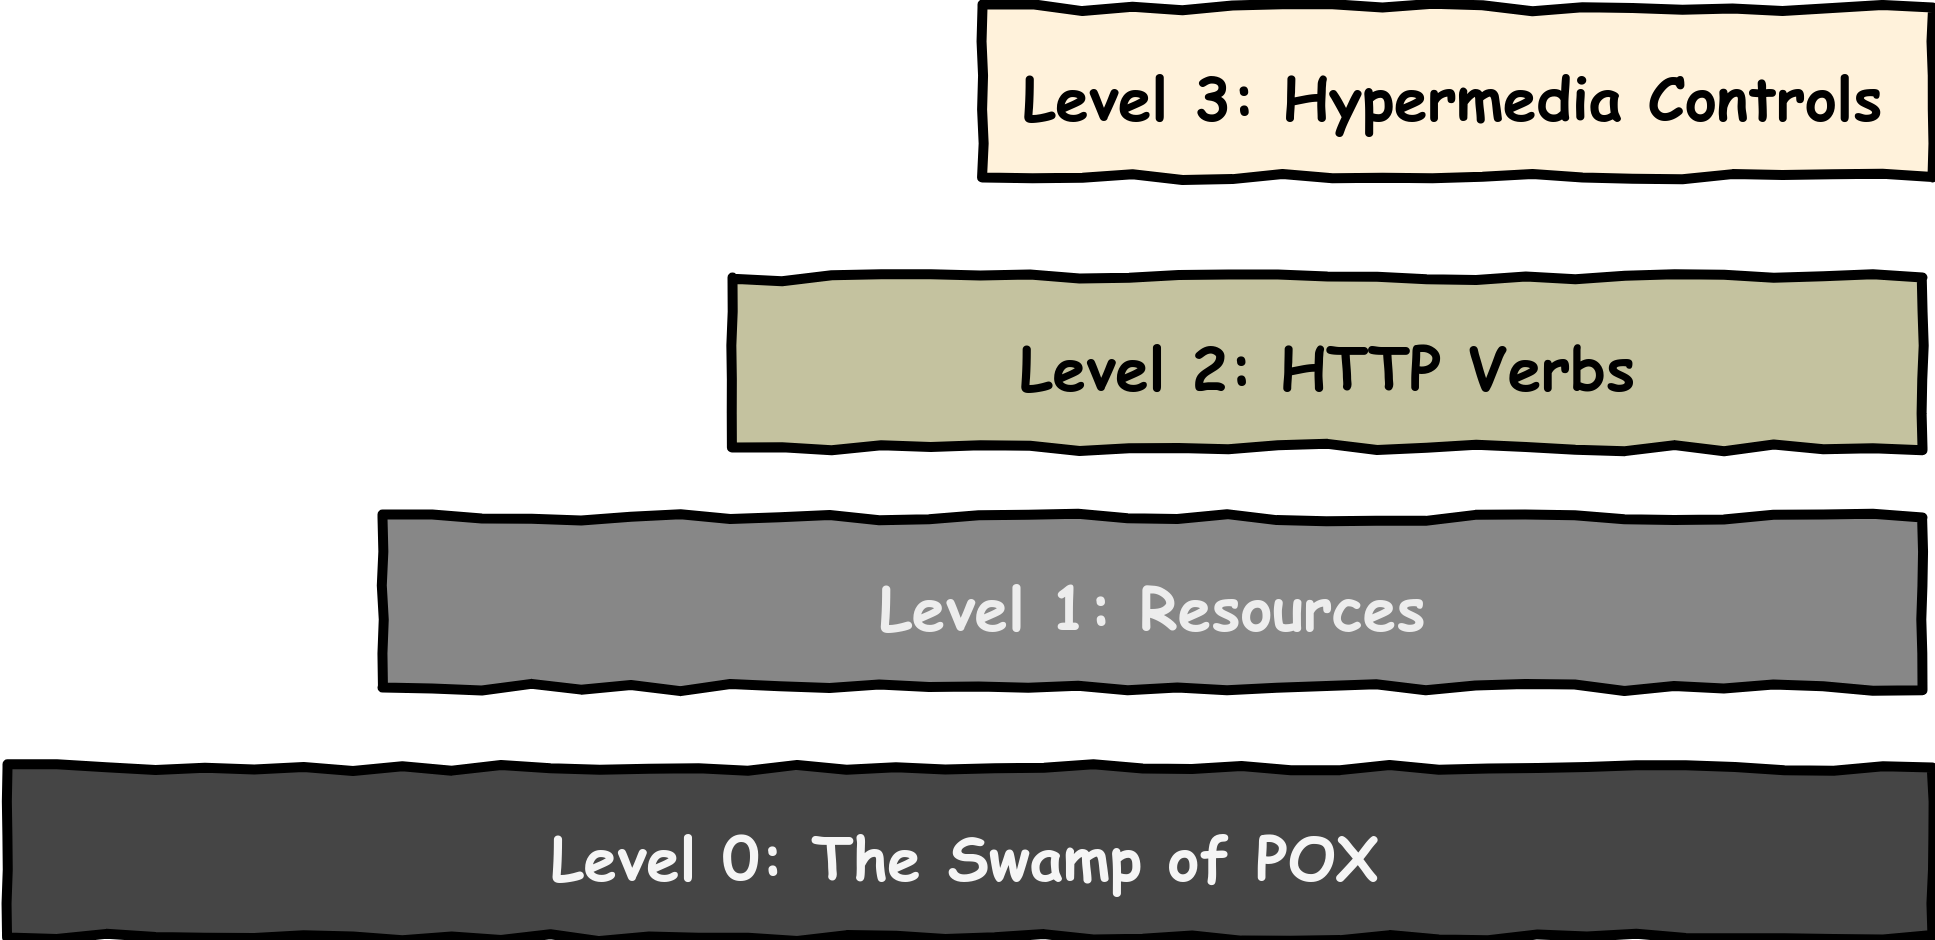
\includegraphics[width=350pt]
    {images/rmm.png}}
  \caption{Steps towards REST. (Source: https://martinfowler.com/articles/richardsonMaturityModel.html)}
\end{figure}

The Richardson Maturity Model describes steps towards REST starting from HTTP. We go through the levels starting with level 0 by looking at an example of a system that allows us to book appointments with our doctor.

\subsubsection{Level 0: The Swamp of POX}

Level 0 uses HTTP as transport system for remote interactions. No other feature of the web are used and HTTP is only used for tunneling requests. SOAP or GraphQL work on this level. \\
To book an appointment at our doctor we create following request:

\lstset{language=XML}
\begin{lstlisting}[caption=Level 0: Remote procedure call on HTTP]
POST /appointmentService HTTP/1.1
[various other headers]

<openSlotRequest date = "2010-01-04" doctor = "mjones"/>
\end{lstlisting}

\subsubsection{Level 1: Resources}

Level 1 introduces the concept of resources. Instead of referring to the doctor within our request we encode the doctor in the URL. This is similar the the concept of an object identity, where an object instance can be identified by an id.

\lstset{language=XML}
\begin{lstlisting}[caption=Level 1: Referring to the doctor as a resource.]
POST /doctors/mjones HTTP/1.1
[various other headers]

<openSlotRequest date = "2010-01-04"/>
\end{lstlisting}

\subsubsection{Level 2: HTTP Verbs}

Level 2 introduces HTTP verbs like \lstinline{GET}, \lstinline{POST} or \lstinline{DELETE}. Instead of using \lstinline{POST} everywhere, we choose the most specific verb that fits the use case as defined by HTTP.
Fowler puts the emphasis here on \lstinline{safety} and says that it is not too important to make use of all the HTTP verbs. Proper use of the safe and idempotent verb \lstinline{GET} and the unsafe verb \lstinline{POST} improves an API a lot according to him. \\
Level 2 additionally adds the proper use of HTTP status codes. The creation of a resource using \lstinline{POST} should return the HTTP status code \lstinline{201 Created}.

\lstset{language=}
\begin{lstlisting}[caption=Level 2: Safely fetching the list of open slots using \lstinline{GET}.]
GET /doctors/mjones/slots?date=20100104&status=open HTTP/1.1
Host: royalhope.nhs.uk
\end{lstlisting}

\subsubsection{Level 3: Hypermedia Controls}

The final level introduces something that you often hear referred to under the ugly acronym of HATEOAS (Hypertext As The Engine Of Application State). It addresses the question of how to get from a list open slots to knowing what to do to book an appointment. \citep{richardsonmaturitymodel}

We begin with the known request to get the list of open slots:

\lstset{language=}
\begin{lstlisting}[caption=Fetching the list of open slots.]
GET /doctors/mjones/slots?date=20100104&status=open HTTP/1.1
Host: royalhope.nhs.uk
\end{lstlisting}

The response has has the URIs that help us understand how to book an appointment.

\lstset{language=}
\begin{lstlisting}[caption=Level 3: The response contains information that helps us to book an appointment.]
HTTP/1.1 200 OK
[various headers]

<openSlotList>
  <slot id = "1234" doctor = "mjones" start = "1400" end = "1450">
     <link rel = "/linkrels/slot/book"
           uri = "/slots/1234"/>
  </slot>
  <slot id = "5678" doctor = "mjones" start = "1600" end = "1650">
     <link rel = "/linkrels/slot/book"
           uri = "/slots/5678"/>
  </slot>
</openSlotList>
\end{lstlisting}

Still, there is ambiguity and the client (we) need some prior knowledge on how to book an appointment.

\subsubsection{Level 4: Linked data driven UI for task-based computing}

This thesis describes Level 4.

\begin{figure}[!htb]
  \center{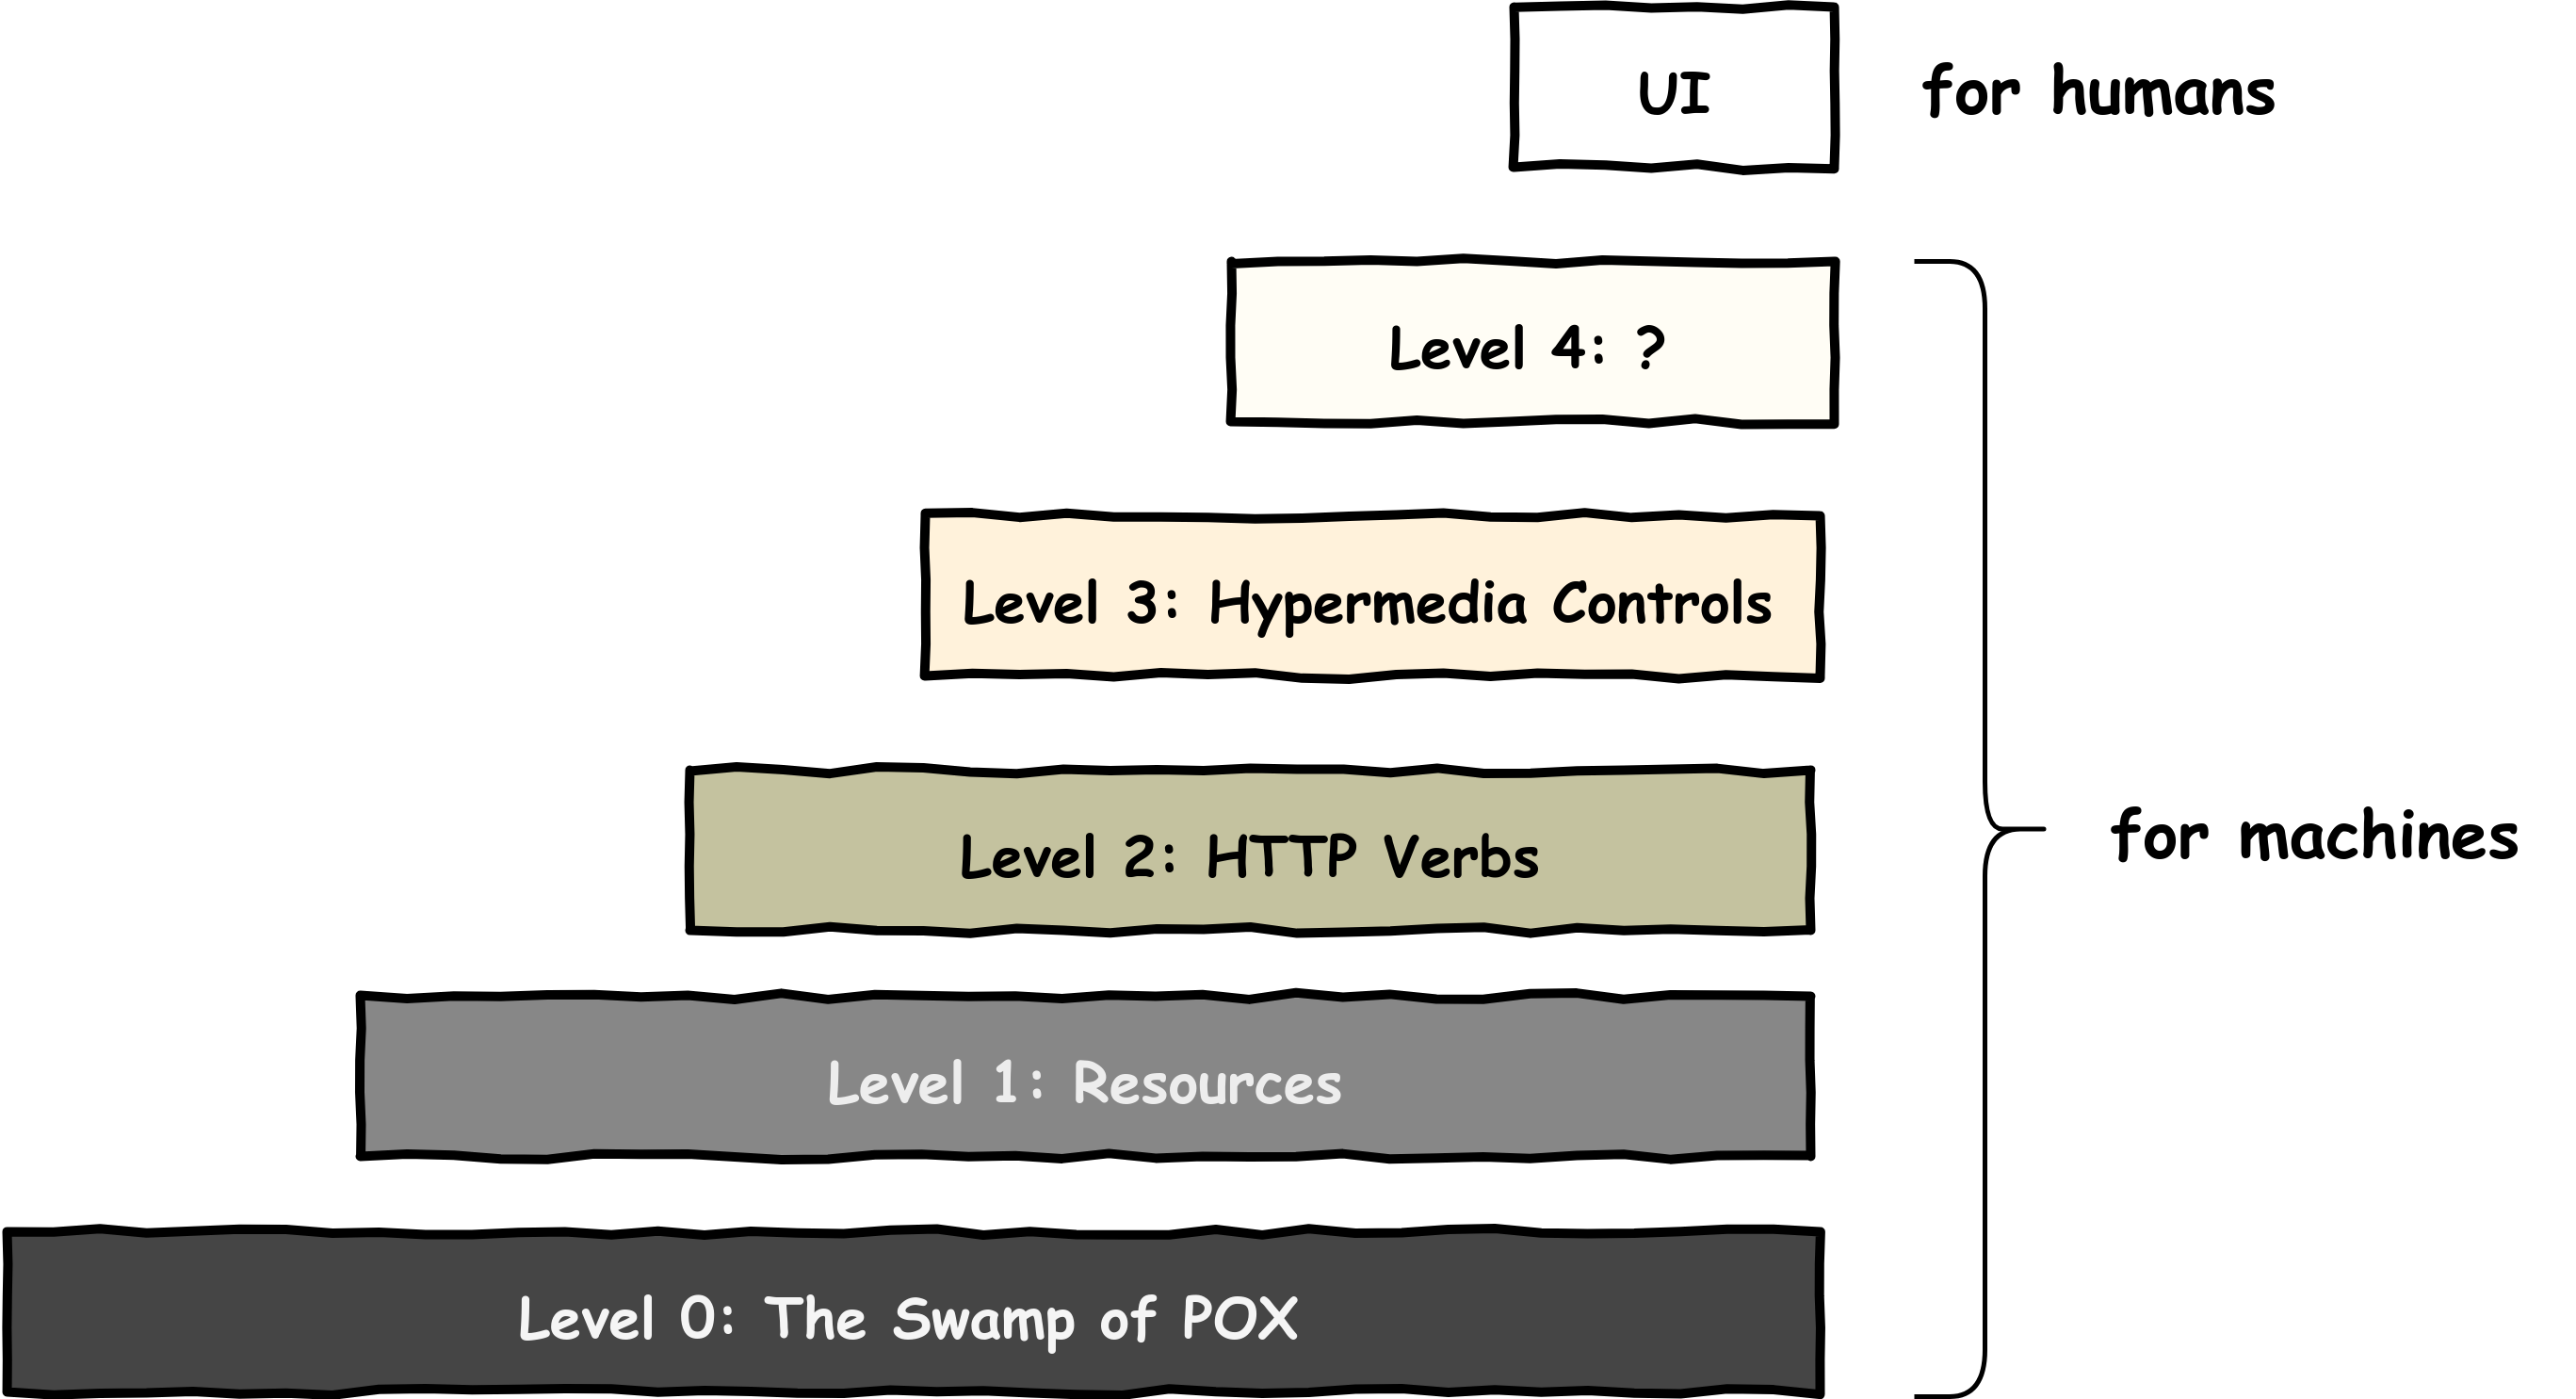
\includegraphics[width=380pt]
    {images/rmm-next.png}}
  \caption{From REST to UI. (Source: https://martinfowler.com/articles/richardsonMaturityModel.html)}
\end{figure}

\subsection{Linked data}\label{linkeddata}

Linked data is a way of creating a web of machine interpretable data across different domains, systems and organizations. A person or a machine should be able to explore data by simply following links. In essence, the same expectations apply to make that web of data grow as to linked HTML documents: \citep{linkedatafourrules}

\begin{enumerate}
  \item Use URIs as names for things
  \item Use HTTP URIs so that people can look up those names.
  \item When someone looks up a URI, provide useful information, using the standards (RDF*, SPARQL)
  \item Include links to other URIs, so that they can discover more things.
\end{enumerate}

A machine looking at a piece of linked data follows the links and is able to unambiguously understand the data. This is equivalent of traversing a graph since linked data is effectively a giant graph. There are multiple serialization formats in the family of specifications called Resource Description Framework (RDF) \citep{rdfspecification}.

An RDF file describing a Smith family could live at \lstinline{http://example.org/smith} and have following content:

\lstset{language=XML}
\begin{lstlisting}[caption= Simple example of a person as RDF, label=rdfexample]
<rdf:Description about="#albert"
 <fam:child rdf:Resource="#brian">
  <fam:child rdf:Resource="#carol">
  </rdf:Description>
\end{lstlisting}

Information about the grandparent Albert can be obtained by loading the data at \\ \lstinline{http://example.org/smith#albert}. Albert's child Brian can be accessed at \\  \lstinline{http://example.org/smith#brian} and Brian's child Carol at \lstinline{http://example.org/smith#carol}.

\subsection{JSON-LD}\label{jsonld}

In web development the main format for data exchange now is JSON \citep{jsonformat}. It is easy to parse, to generate, arguably easier for humans to read than XML and many languages provide first-class support for it.

However, JSON is difficult to integrate from different sources as the data may contain keys that conflict with other data sources. JSON has no built-in support for hyperlinks, which are a fundamental building block on the Web \citep{jsonldbasicconcepts}. It doesn't provide any means to attach meta data to the data itself and one has to use other mechanisms to provide meta data like HTTP headers.

Consider following JSON snippet:

\lstset{language=JSON}
\begin{lstlisting}[caption=Data of a person in the JSON format, label=jsonexample]
{
  "name": "Manu Sporny",
  "homepage": "http://manu.sporny.org/",
  "image": "http://manu.sporny.org/images/manu.png"
}
\end{lstlisting}

It's obvious to humans that the data is about a person whose name is \textit{Manu Sporny} and that the homepage property contains the URL of that person's homepage. A machine doesn't have such an intuitive understanding and sometimes, even for humans, it is difficult to resolve ambiguities in such representations. This problem can be solved by using unambiguous identifiers to denote the different concepts instead of tokens such as \textbf{name} or \textbf{homepage} \citep{jsonldbasicconcepts}.

JSON-LD is a serialization format for linked data and is based on JSON-LD. By using the popular schema.org vocabulary the example \ref{jsonexample} can be written as follows:

\lstset{language=JSON}
\begin{lstlisting}[caption=Data of a person in the JSON-LD format, label=jsonldexample]
{
  "http://schema.org/name": "Manu Sporny",
  "http://schema.org/url": {
    "@id": "http://manu.sporny.org/"
  },
  "http://schema.org/image": {
    "@id": "http://manu.sporny.org/images/manu.png"
  }
}
\end{lstlisting}

This can be understood by any machine without providing additional information. The key \lstinline{http://schema.org/name} can be looked up to determine the meaning of the value \lstinline{Manu Sporny}. JSON-LD supports the concept of a \textbf{context}.

The context is meta data that has to be provided together with the data. This makes it possible for a machine to attach meaning to it. Thanks to the context it is not required to have the keys as absolute URIs anymore. The data can be compacted and written as follows:

\lstset{language=JSON}
\begin{lstlisting}[caption=Compacted data of a person, label=jsonldcompacted]
{
  "@context": "http://schema.org",
  "name": "Manu Sporny",
  "url": "http://manu.sporny.org/",
  "image": "http://manu.sporny.org/images/manu.png"
}
\end{lstlisting}

With the small addition of the reserved keyword \lstinline{@context} readability of JSON was restored while allowing machines to understand the data. JSON-LD is 100\% compatible with JSON and therefore benefits of the vast amount of JSON tooling available.


\subsubsection{JSON-LD and the Semantic Web}
The concepts of the Semantic Web were formed in the 1960s as something called \textbf{semantic network}. The technologies that power the Semantic Web today appeared in the 2000s. In 2006 Tim Berners-Lee, inventor of the World Wide Web, stated that the simple idea of the Semantic Web remains largely unrealized \citep{semanticwebrevisited}.

JSON-LD became official standard in 2014, a few years after the core technologies of the Semantic Web emerged. As opposed to the Semantic Web and its technologies JSON-LD has seen a widespread adoption in the software industry. Among the users of JSON-LD are Microsoft, Google, Yandex and a few Apache projects \citep{jsonldusers}. Both the technologies of the Semantic Web and JSON-LD are concerned with linked data. Why is JSON-LD experiencing adoption?

Manu Sporny, one of the primary creators of JSON-LD, criticizes the Semantic Web in his blog post \textit{JSON-LD and why I hate the Semantic Web}. His criticism has two aspects.

\paragraph{Social}
The main point of his criticism is that the Semantic Web working group neglects the human factor in software development. The goal of widespread adaption in mainstream web development can not be achieved if it requires the setup of a SPARQL engine, quad store and other RDF tooling. The average web developer has no interest dealing with this overhead. He further critiques the W3C specifications and states that they are hard to read. \citep{semanticwebrevisited} Manu further mentions how the Semantic Web community creates esoteric solutions to non-problems. \citep{semanticwebrevisited}

\paragraph{Technology}
The second point is criticism on the technological decisions mainly about RDF. RDF has no native support for lists it didn't have support for graphs for a long time. One of the goals was to remain compatible to RDF with JSON-LD, so that data can be serialized and deserialized from and to each other. \citep{semanticwebrevisited}

\subsubsection{JSON-LD Operations}
There are a few operations that can be executed on JSON-LD. Following are the three most important ones for this thesis.

\paragraph{Framing}

Framing is an operation that re-shapes the data. Input of the framing operation is data and a \textbf{frame}. The frame determines the new shape of the data.

Consider following data of a library. The data is in the form of a normalized graph. The \lstinline{contains} relation represents edges between nodes, the items in the \lstinline{@graph} list are the graph nodes.

\lstset{language=JSON}
\begin{lstlisting}[caption=Data of a library as normalized graph]
{
  "@context": {
    "@vocab": "http://example.org/",
    "contains": {"@type": "@id"}
  },
  "@graph": [{
    "@id": "http://example.org/library",
    "@type": "Library",
    "contains": "http://example.org/library/the-republic"
  }, {
    "@id": "http://example.org/library/the-republic",
    "@type": "Book",
    "creator": "Plato",
    "title": "The Republic",
    "contains": "http://example.org/library/the-republic#introduction"
  }, {
    "@id": "http://example.org/library/the-republic#introduction",
    "@type": "Chapter",
    "description": "An introductory chapter on The Republic.",
    "title": "The Introduction"
  }]
}
\end{lstlisting}

Following frame determines the shape of the frame data:

\lstset{language=JSON}
\begin{lstlisting}[caption=Frame for the framing operation]
{
  "@context": {
    "@version": 1.1,
    "@vocab": "http://example.org/"
  },
  "@type": "Library",
  "contains": {
    "@type": "Book",
    "contains": {
      "@type": "Chapter"
    }
  }
}
\end{lstlisting}

The result of the framing operation is a tree:

\lstset{language=JSON}
\begin{lstlisting}[caption=Framed data of a library]
{
  "@context": {
    "@version": 1.1,
    "@vocab": "http://example.org/"
  },
  "@id": "http://example.org/library",
  "@type": "Library",
  "contains": {
    "@id": "http://example.org/library/the-republic",
    "@type": "Book",
    "contains": {
      "@id": "http://example.org/library/the-republic#introduction",
      "@type": "Chapter",
      "description": "An introductory chapter on The Republic.",
      "title": "The Introduction"
    },
    "creator": "Plato",
    "title": "The Republic"
  }
}
\end{lstlisting}

\paragraph{Compacting}\label{jsonldcompacting}

Compacting describes the operation of reducing verbosity in the JSON-LD data. Compacted data is meant to be read and understood by human developers. This is achieved by pulling out the context and explicitely define it using the \lstinline{@context} keyword.

Consider following input:

\lstset{language=JSON}
\begin{lstlisting}[caption=Verbose data of a person]
{
  "http://schema.org/name": "Manu Sporny",
  "http://schema.org/url": {
    "@id": "http://manu.sporny.org/"
  },
  "http://schema.org/image": {
    "@id": "http://manu.sporny.org/images/manu.png"
  }
}
\end{lstlisting}

This data can be compacted by pulling out the \lstinline{@context}:

\lstset{language=JSON}
\begin{lstlisting}[caption=Compacted and easy-to-read data of a person]
{
  "@context": "http://schema.org",
  "name": "Manu Sporny",
  "url": "http://manu.sporny.org/",
  "image": "http://manu.sporny.org/images/manu.png"
}
\end{lstlisting}

\paragraph{Expanding}\label{jsonldextending}

Expanded data serves the opposite goal of compacting data. While compacted data is easy to read for humans, extended data is easy to process for machines.

Expanding the following compacted data

\lstset{language=JSON}
\begin{lstlisting}[caption=Compacted and easy-to-read data of a person]
{
  "@context": "http://schema.org",
  "name": "Manu Sporny",
  "url": "http://manu.sporny.org/",
  "image": "http://manu.sporny.org/images/manu.png"
}
\end{lstlisting}

results in following expanded data:

\lstset{language=JSON}
\begin{lstlisting}[caption=Expanded data of a person that is easy to process for machines]
[
  {
    "http://schema.org/image": [
      {
        "@id": "http://manu.sporny.org/images/manu.png"
      }
    ],
    "http://schema.org/name": [
      {
        "@value": "Manu Sporny"
      }
    ],
    "http://schema.org/url": [
      {
        "@id": "http://manu.sporny.org/"
      }
    ]
  }
]
\end{lstlisting}

\subsection{Vocabulary}

JSON-LD is essentially a linked data serialization format that plays well with JSON tooling. Creating linked data means creating a vocabulary that other might use by linking to it. A lot of vocabularies those exist and two of them are particularly interesting for this thesis.

\subsubsection{Schema.org}

\url{Schema.org} is a collaborative, community activity with a mission to create, maintain, and promote schemas for structured data on the Internet, on web pages, in email messages, and beyond \citep{welcomeschemaorg}. Companies like Google, Microsoft, Pinterest and Yandex are using it in their tools and products.

Their main goal is to provide a shared vocabulary that web developers can refer to. It is often used in the context of search engine optimization by helping crawlers understand websites.

Schema.org is a hierarchy of \lstinline{Things} that have an implicit \textbf{is a} relationship. This is similar to sub typing through inheritance in many object-oriented programming languages. Following is a small subset of the Schema.org hierarchy:

\begin{figure}[!htb]
  \center{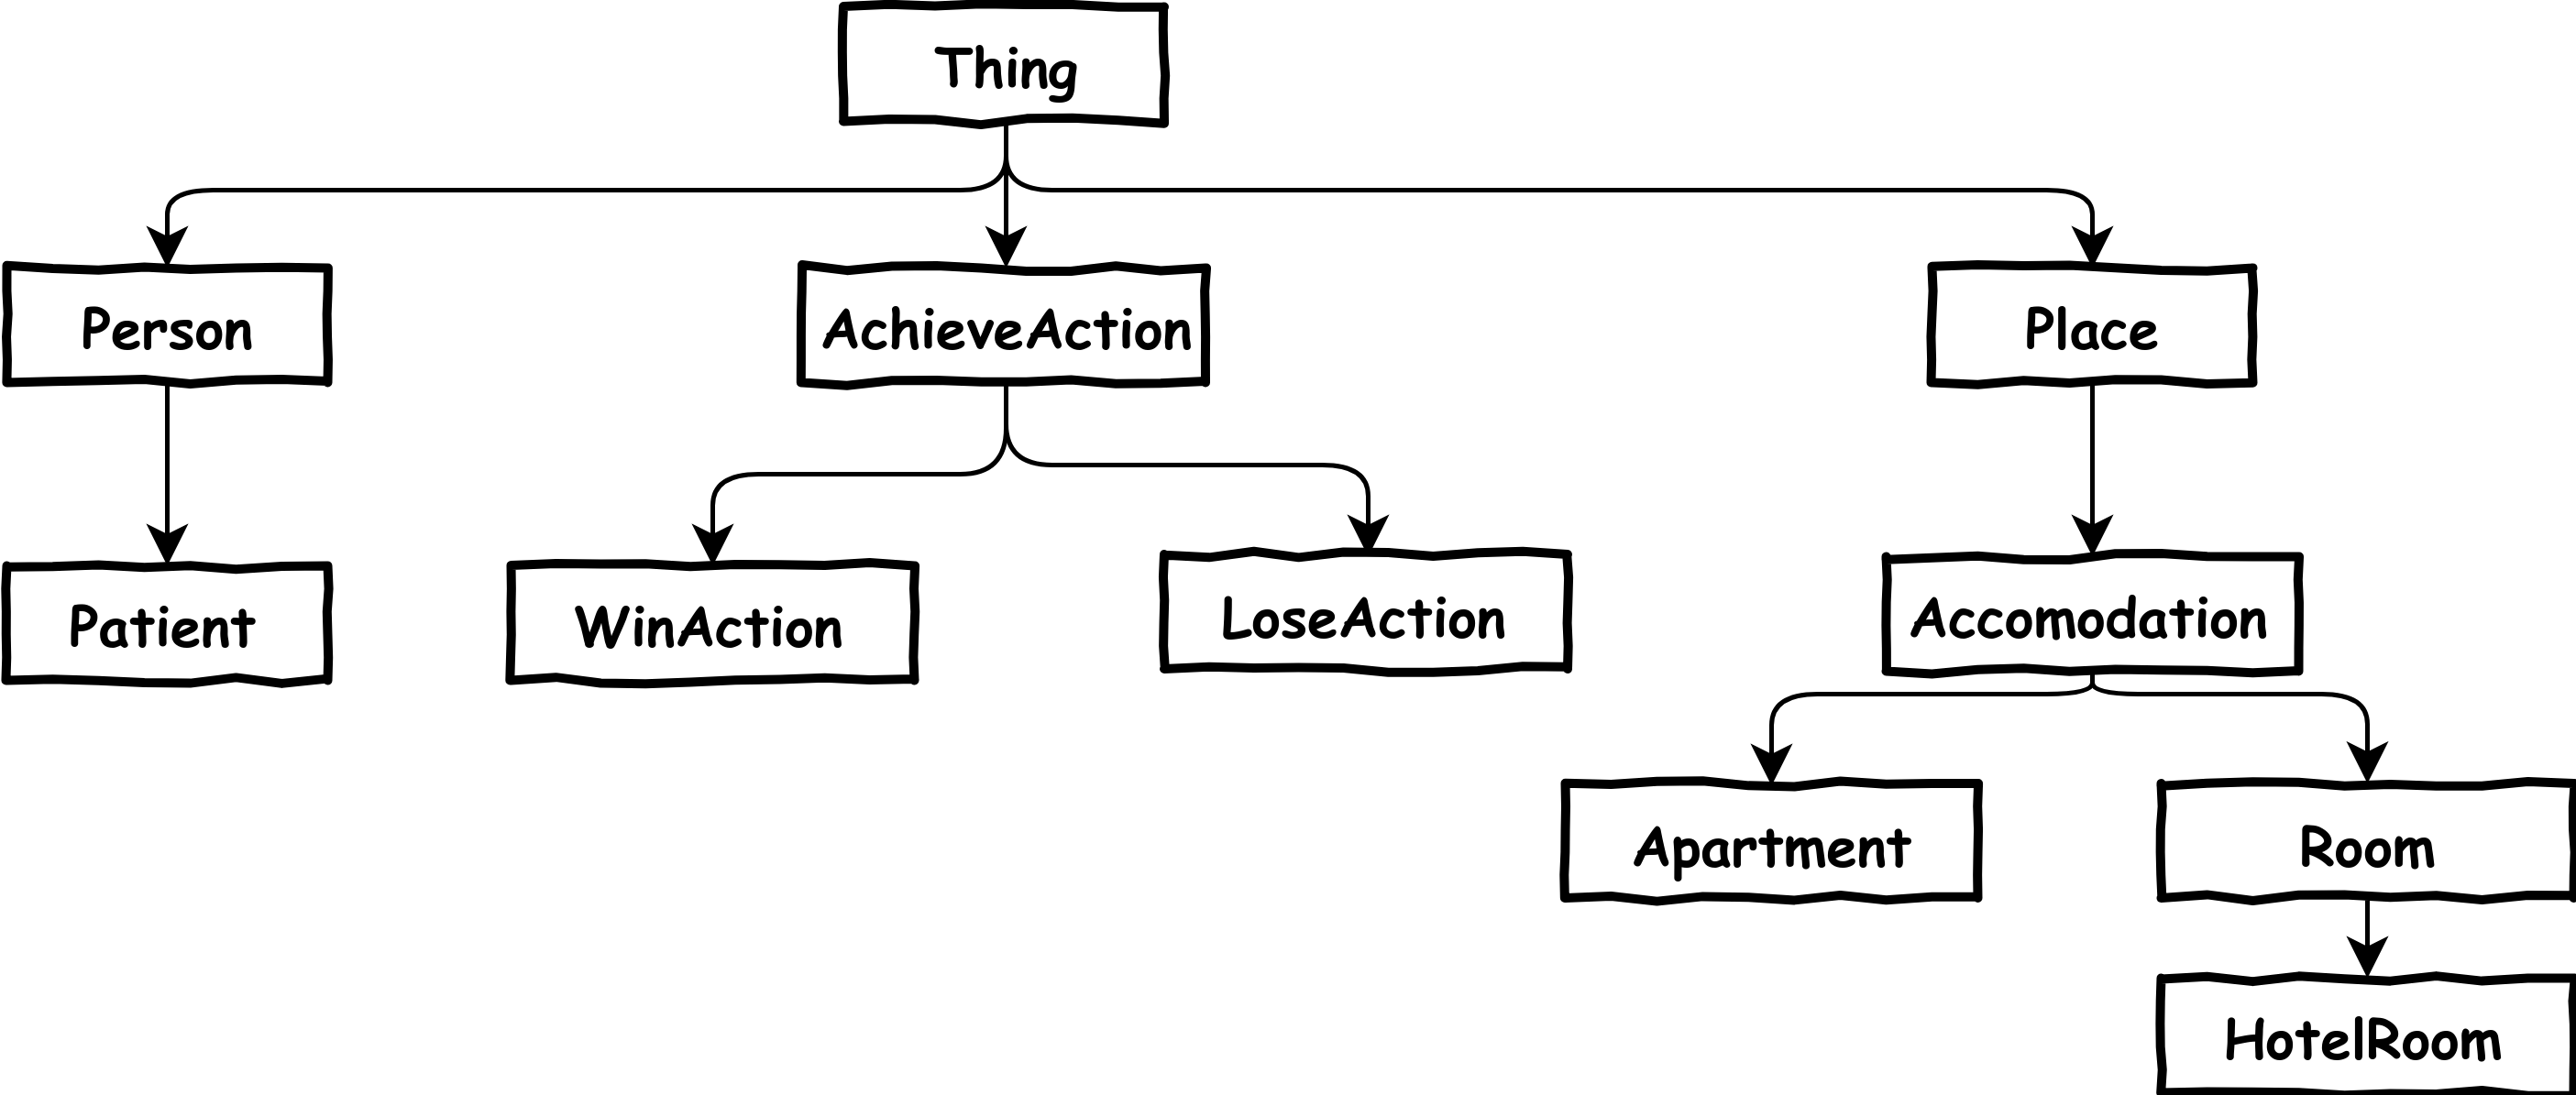
\includegraphics[width=380pt]
    {images/schemaorg.png}}
  \caption{\label{fig:schemaorg} Subset of the Schema.org ontology where child-parent relation describes an \textit{is a} relationship.}
\end{figure}

The advantage of using such a vocabulary becomes obvious when looking at an example.The type \lstinline{Person} has a property \lstinline{address}. \lstinline{Address} can be of type \lstinline{http://schema.org/Text} or \lstinline{http://schema.org/PostalAddress}.

\lstset{language=JSON}
\begin{lstlisting}[caption=A person with an address of type Text]
{
  "@context": "http://schema.org",
  "givenName": "Walter",
  "familyName": "White",
  "address": "3828 Piermont Dr NE Albuquerque, NM 87111, USA"
}
\end{lstlisting}

A machine receiving that data knows that this is a person and understands his name, but it can not understand his address. There is additional context needed that describes the schema used in the \lstinline{address} property.

The data of the same person where the address is of type \lstinline{http://schema.org/PostalAddress} can be processed unambiguously by any machine that understands linked data.

\lstset{language=JSON}
\begin{lstlisting}[caption=A person with an address of type PostalAddress]
{
  "@context": "http://schema.org",
  "givenName": "Walter",
  "familyName": "White",
  "address": {
    "@type": "PostalAddress",
    "addressLocality": "Albuquerque",
    "addressRegion": "NM",
    "postalCode": "87111",
    "streetAddress": "3828 Piermont Dr NE Albuquerque"
  },
}
\end{lstlisting}

The \lstinline{streetAddress} is still stringly typed. A system running at a package distribution center could route packages correctly to some local distribution center or postal office by looking at \lstinline{addressRegion} and \lstinline{addressLocality}.

\subsection{Contemporary solutions and tools}
In this section we discuss solutions and tools that claim to reduce complexity and enhance efficiency in software development and especially in UI development. \\ For each tool we discuss its benefit and analyze how it can be used to reduce decrease development costs.

\subsubsection{SOAP}
SOAP Version 1.2 (SOAP) is a lightweight protocol intended for exchanging structured information in a decentralized, distributed environment. It uses XML technologies to define an extensible messaging framework providing a message construct that can be exchanged over a variety of underlying protocols. The framework has been designed to be independent of any particular programming model and other implementation specific semantics \citep{soap}. \\ It is popular in large enterprises because it works well in a distributed setting and it has certain security and safety mechanisms built in. In general web development REST with JSON has superseded SOAP because it brings less complexity and is more flexible.

In order to work with SOAP one has to use XML, which is harder to parse, generate and read than JSON. In contrast to XML, JSON provides no means to attach meta data. \\
Because REST is more of an architectural style than an architecture, there are multiple ways to achieve do certain things.

\subsubsection{GraphQL}\label{graphql}
GraphQL is a query language for APIs and a set of tools to fulfill those queries \citep{graphql}. It provides a way to define the data model as graph that can be queried and mutated. There is a growing ecosystem consisting of tools for implementing GraphQL servers and GraphQL clients.

\lstset{language=GraphQL}
\begin{lstlisting}[caption=Simple data model in the GraphQL data description language.]
type Project {
  name: String
  tagline: String
  contributors: [User]
}
\end{lstlisting}
\lstset{language=GraphQL}
\begin{lstlisting}[caption=Example of a GraphQL query to fetch the tagline of a certain project.]
{
  project(name: "GraphQL") {
    tagline
  }
}
\end{lstlisting}
\lstset{language=JSON}
\begin{lstlisting}[caption=Response of the GraphQL server in JSON.]
{
  "project": {
    "tagline": "A query language for APIs"
  }
}\end{lstlisting}

GraphQL mitigates the problem of over and under fetching. The client tells the server the structure of the data it expects by defining which parts are interesting. The server takes of denormalization and send the client exactly the data it requested. \\ This makes GraphQL very popular for mobile app development where the bandwidth is often limited. Another benefit of this approach is that the data model and the usage of the data by the client is decoupled. The client doesn't have to do any processing or additional fetches, which is beneficial on mobile devices.
GraphQL provides a way of self-documentation through introspection. Developers are able to use the same query mechanisms for data and for documentation meta data, which makes exploration of such an API trivial. This requires additional tooling that for instance queries the valid fields of an entity to suggest field names to a developer that is writing the query.

However, GraphQL completely disregards existing HTTP and JSON tooling. As mentioned in section \ref{richardsonmaturitymodel}, Level 1 introduces HTTP resources. GraphQL ignores this step and builds on top of Level 0 by merely using HTTP as transport system. This renders HTTP caching useless and tools that assume JSON as data exchange format require additional effort to work with GraphQL. \\ The introduction of a new language requires syntax highlighting in editors. \\ In order to make use of self-documentation the GraphQL editor has to query the GraphQL schema that has to be provided by the server and kept up-to-date.

The adoption of GraphQL is not a small commitment. Since it doesn't build on top of existing standards and tools there is no upgrade path from an existing RESTful API. If an organization, a department or a team decides to adopt GraphQL and to use it over REST, it can speed up UI and client development and it can decrease maintenance costs. However GraphQL can only be used in that context as \textbf{it doesn't play well with others}. This could lead to isolated GraphQL servers where the data exchange with non-GraphQL servers suffers from friction.

Additionally GraphQL provides no means to a generic client to build operations. This makes it unusable as hypermedia technology.

\subsubsection{Rails with ActiveAdmin}
Ruby on Rails is a web framework that emerged in the 2000s and influenced the way web applications are built today \citep{rubyonrails}. Rails allows rapid application development by following a Convention over Configuration philosophy. This makes Rails a strongly opinionated framework that guides development by providing \textbf{sane but overrideable defaults}.

ActiveAdmin is an add-on for Rails that comprises a DSL to define admin UIs. The main use case of ActiveAdmin is the creation of applications for administrators. These UIs don't have the strict esthetic requirements that customer facing ones have. They just to expose all necessary operations of an application so that administrators can fulfill their duties. \\ ActiveAdmin directly leverages the data model of a Rails application and it knows the Rails conventions. The use of a UI specific DSL and the fact that ActiveAdmin knows the domain model allow UI developers to quickly bootstrap applications for administrators.

The strong coupling to Rails is its major weakness. While ActiveAdmin reduces UI development costs immensely, it does so in that small world. The assumptions it makes about the server prevents it to support distributed data models in an idiomatic way. As soon as there are multiple Rails instances contributing to one data model, ActiveAdmin is no longer useful.

Being an add-on to Rails ActiveAdmin doesn't not work outside of the Rails ecosystem.

\subsection{Industrial partner}
TODO
